The same optimizations as well as trade-offs between performance, power and energy discussed for the lazy shadowing of a single task can be applied in the case of $M$ tasks,
as long as the tasks execute independently without synchronization. If execution is divided into phases with synchronization only between phases, then a global optimization may be also formulated by applying a local optimization within each phase.
The behavior within one phase in which each task executes $W$ units of work is still captured by Figure~\ref{fig:sync}. Specifically, with $M$ tasks,
Figure~\ref{fig:sync}(b) illustrates the behavior of any main/shadow pair when the main fails at time $t_f$ after which time the shadow
executes at maximum rate. Figure~\ref{fig:sync}(a) illustrates the behavior of all other main/shadow pairs that continue execution, not necessarily aware of the failure. However, because the tasks have to synchronize after each one executes $W$ units of work, then all the mains that did not fail will reach that synchronization point at time $t_m$ while the shadow of the faulty main will reach that point at a later time $t_s$.  Hence, the non-faulty mains will be idle from $t_m$ until $t_s$.

Clearly, the inefficiency implied by the non-faulty mains waiting for the shadow of a faulty main at a synchronization point becomes more acute when synchronization points are frequent, which is the case in many HPC applications. Hence, we will concentrate in the rest of this paper on shadowing for tasks that are tightly coupled, corresponding to the computational model in Section~\ref{sec:com_model}. Specifically, we will assume that time between synchronizations is very small compared to the total execution time. Consequently, if one main, M(i), fails at time $t_f$, then other mains will have to wait for S(i) very soon after $t_f$ (at time $t_m = t_f+\epsilon$, where $\epsilon \to 0$).

\begin{figure}[!t]
	\begin{center}
			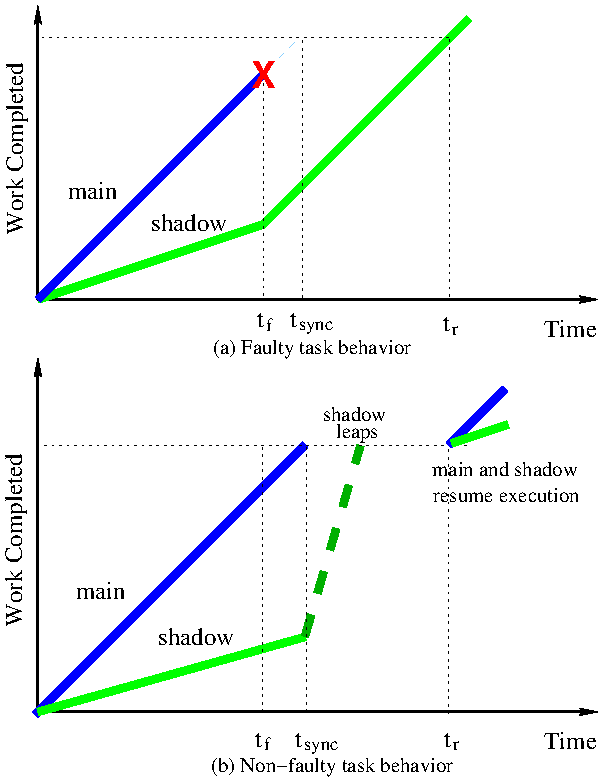
\includegraphics[width=0.8\columnwidth]{Figures/jump.pdf}
	\end{center}
	\vskip -0.25in
	\caption{The concept of Leaping Shadows.}
	\label{fig:leap}
\end{figure}

The waiting time, $t_w$ = $t_s - t_m$ = $(1-\sigma_s^b)t_f$, is caused by the fact that $\sigma_s^b < 1$. To utilize the waiting time between $t_m$ and $t_s$ effectively, we propose to align the state of the shadows with those of the corresponding mains after each failure, using Direct Remote Memory Access (RDMA). We call this technique \emph{leaping shadows}. Specifically, for the shadows associated with the non-faulty mains, each of them updates its state by rolling forward to the state of its main. This way, after the synchronization point, every main and its shadow will resume execution from the same consistent state, as shown in Figure~\ref{fig:leap}.  %Clearly the waiting time, $t_w$ increases with $t_f$ and $S$. The time for the $S$ shadows in a shadowed set to update their states (leap) to match the states of their corresponding mains increases with $S$, and with the difference between the states of the mains and shadows, which increases with $t_f$. We will study this relation thoroughly, keeping in mind that the size of shadowed group, $S+1$, may be constrained by the requirement that all $S$ shadows in a group can leap within the period, $t_w$.